\chapter{Experiments}
\label{chap:experiments}
In this chapter, we elaborate on the dataset used with our model, how we fine-tuned our parameters and the different metrics and method we used to evaluate our solution. We then introduce both qualitative and quantitative results and discuss them.

\section{Experimental protocol}
\label{section:protocol}
In this section, we describe our experimental protocol and introduce the evaluation methods we use.

\subsection{Datasets}
As detailed in chapter \ref{chap:archi}, we use two distinct datasets for our action recognition process. The first one serves as input to the original SOINN model and use preprocessed human body pose estimation frames as input. The body pose estimation is given by OpenPose, but we needed to define a good dataset from which we extract these poses. After a few surveys, we chose to use Hollywood in Homes (HiH) \cite{HiH}. It is a crowdsourced dataset with the following characteristics:

\begin{itemize}
    \item{Composed of 9846 unlabeled videos filmed at 30 frames per second.}
    \item{Average length for each video: 25 seconds.}
    \item{Videos describe everyday indoor scenes in private housing.}
    \item{Typically recorded using smartphone, providing an amateur look that approach typical 2D robot vision perspective.}
    \item{Extremely diverse in terms of subjects, environment, activities, camera angle, lightning conditions, ...}
\end{itemize}
An example of random frames taken from HiH is displayed in figure \ref{fig:HiH}.

\begin{figure}[htp]
\centering
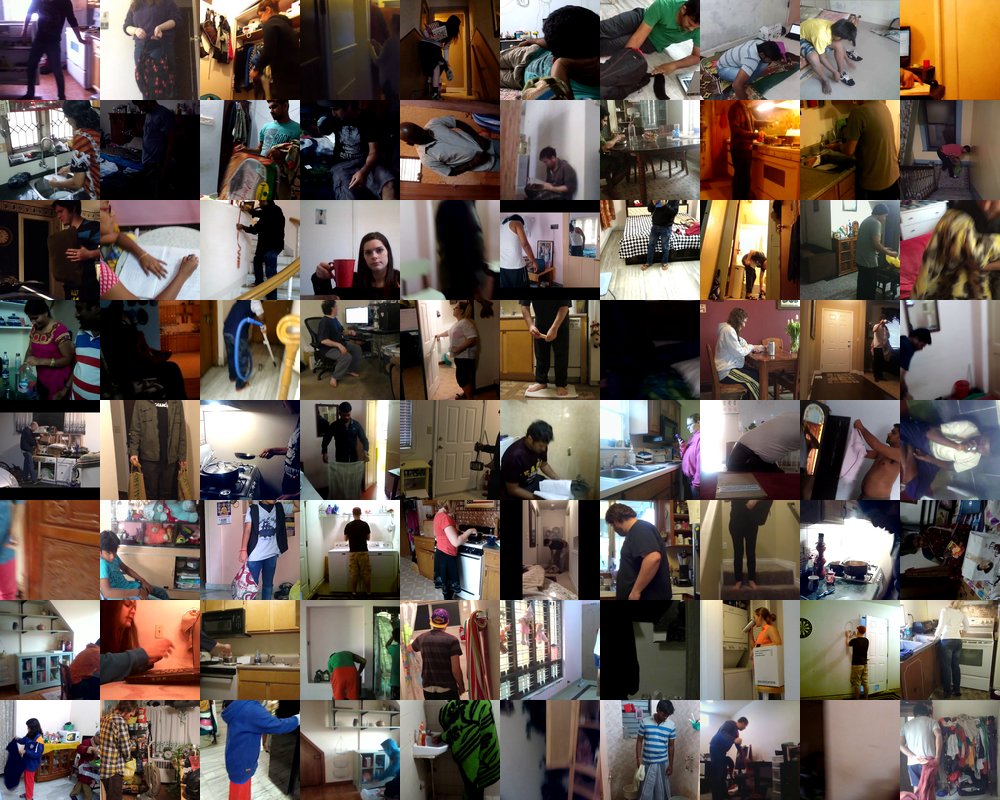
\includegraphics[width=120mm, keepaspectratio]{images/HiH.png}
\caption{Random frames taken from Hollywood in Homes dataset.}
\label{fig:HiH}
\end{figure}

In order to test our method efficiency, we tried its implementation on our turtlebot. We recorded one individual performing a few actions in a small indoor environment. After performing object detection, about 10 objects were detected in that environment and we recorded 23 interaction during the 30 seconds long experiment.

\textbf{COMPLETE HERE}

\subsection{Metrics used}
It is often difficult to evaluate an unsupervised clustering algorithm. In supervised classification, a natural metric is average accuracy, where the accuracy is simply the proportion of well classified examples, with examples taken from a labeled dataset where we know the ground truth. For unsupervised clustering, the algorithm separates data in clusters but do not issue a label for these clusters. 

Nevertheless, it is sometimes possible to evaluate them by using a labeled dataset from which we hide the labels to the algorithm during training, and we can then compare the outputs of the algorithm with the ground truth labels by several means. However this type of evaluation technique is only possible if we have labeled data to use. Unfortunately, it is not the case in our study, since our original dataset is unlabeled and our refined algorithm makes use of data that is personal to the robot. 

For these reasons, we only have access to a few metrics that do not involve any ground truth comparison. The first one that can be considered is called the relative size of the model $N_{rel}$. It is simply defined as the number of nodes output by the algorithm divided by the size of the training set for a cluster model C: 

\begin{equation}
    N_{rel}(C) = \frac{|C|}{size_{train}(C)}
\end{equation}

$N_{rel}$ is basically the reduction power of the algorithm, it represents its capacity to summarize its input. However, it gives no indication about the quality of that summarize.

In order to evaluate this quality, we introduce another classical evaluation metrics: the Sum of Squared Errors (SSE)\cite{sse-silhouette}. SSE is defined by:

\begin{equation}
    SSE(C) = \sum_{i=1}^k\sum_{o \in C_i}d(o, cen_{i})^2
\end{equation}

where C is a cluster model output by the algorithm, composed of k clusters $C_i$, and $cen_i$ is the centroid of cluster $C_i$.

SSE basically punishes cluster that are too much spread, it is a good measure complementary to $N_{rel}$.

The last metrics available for data without ground truth is the silhouette measure. The silhouette measure of an object $o_i$ assigned to a cluster $C_A$ is:
\begin{equation}
    sil(o_i)= \frac{b(o_i) - a(o_i)}{max\{a(o_i), b(o_i)\}}
\end{equation}
where $a(o_i)$ represents the average distance between $o_i$ and the other objects in the cluster and $b(o_i)$ is the average distance between $o_i$ and the objects in the nearest cluster:

\begin{equation}
    a(o_i) = \frac{1}{|C_A|-1}\sum_{o_j \in C_A, o_j \neq o_i}d(o_i, o_j)
\end{equation}
\begin{equation}
    b(o_i)= \min_{C_B \neq C_A} \frac{1}{|C_B|} \sum_{o_j \in C_B}d(o_i, o_j)
\end{equation}

From there, we can define the silhouette of a cluster as the average silhouette of its objects:
\begin{equation}
    sil(C_i)=\frac{1}{|C_i|} \sum_{o_j \in C_i}sil(o_j)
\end{equation}

and finally the silhouette of the entire model C:
\begin{equation}
    sil(C)= \frac{1}{k} \sum_{i=1}^k sil(C_i)
\end{equation}

The silhouette measure is interesting since it does not just evaluate the average object/centroid inside distance of each cluster, but mitigates it with the object/centroid distance augmentation if that cluster was to disappear.

\subsection{Parameters fine-tuning}
In this section, we detail the value we chose for the different parameters in our model. We recapitulate the chosen values in table \ref{tab:parameters}.

The SOINN algorithm itself takes two parameters as input: the period at which it deletes nodes $\lambda$ and the maximum age of a neighbourhood relationship between two nodes $\gamma$. When testing SOINN with human poses as input, we observed little influence of $\lambda$ on the result, and $\gamma$ tends to fuse too much nodes at its standard value of 50, however the number of nodes increased dramatically for $10 < \gamma < 20$ so we set it at 30 to find a good compromise.

The pre-processing part of our workflow impose a quality threshold T on the pose estimation of the dataset to be considered as valid training data. When $T > 70\%$, the training becomes really long since a lot of frames in the dataset are not well-estimated. It also make SOINN produce more nodes since he becomes more selective on the slight differences between inputs. However, this is not a good thing for subsequent clustering with unfiltered data: most of the pose estimation received as real-time input are not that precise. This situation then leads our model to overfit.
However if T is too low, it is almost as if we do not require any minimum quality for input frames, which means that our model sometimes learns pure artifacts. We observed that a value of 60\% is the best compromise we found to avoid most part of these issues.

Another thing we have to decide for the pre-training part of our workflow is the size of the pre-training set. If the training set is too small, SOINN is not stable enough to handle unfiltered data of lower quality. On the opposite, a too large training set makes the model too rigid and less likely to be influenced by the add of spatial context information. It also reduces the quality of its nodes. We chose to let SOINN learn from 5000 good body pose detection before make it take unfiltered data as input.

The object detection part of our workflow uses euclidean cluster extraction. We have to specify to it the expected size of detected object by indication a minimum and maximum number of points that can contain an object. This parameter is extremely dependent on the environment, and may need to be adapted in real-time to control the number of detected objects. On our test environment, we obtained best results at $min_{points}=300$ and $max_{points}=10000$ but it may vary at lot from one environment to another.

Finally, our modified SOINN algorithm needs three additional parameters: the bonus and malus used to compute the new distance, and the learning rate $\alpha$. In this work, we chose to set bonus to 0.5 and malus to 2 so that they affect signals in the same way, but that may be tuned better in potential future works. $\alpha$ was added to help the model build confidence in its first inputs. We initially wanted to make it converge to 1 as the model receives more signals, but it did not seem to affect the result, so we kept it at its original value of 2.

\begin{table}[hp]
\centering
\caption{Parameter tuning results}
\label{tab:parameters}
\begin{tabular}{|c|c|c|c|c|c|c|c|c|c|}
    \hline
    Parameter & $\lambda$ & $\gamma$ & T & $N_{train}$ & $min_{points}$ & $max_{points}$ & bonus & malus & $\alpha$ \\
    \hline
    Value & 100 & 30 & 0.6 & 5000 frames & 300 & 10 000 & 0.5 & 2.0 & 2.0 \\
    \hline
\end{tabular}
\end{table}

\subsection{Comparison method}
Since our algorithm now manipulates [pose, interaction] signals instead of normal pose signal of naive pose estimation, it is difficult to evaluate the performance gain that it brings. In order to compare our proposed modified algorithm with naive pose estimation, we will project the outputs to normal body pose space. By doing that, we can compute scores that are comparable with each other using the metrics described earlier. 

However, we should keep in mind that these evaluations only partly represent the gain of information we have from human/object interaction context to the model, and we can only infer that the unprojected model behaves similarly.

\section{Results}
In this section, we show both visual results and numeric evaluation scores computed using methods described in section \ref{section:protocol}.
\subsection{Results visualization}
Showcase of nodes.
\subsection{Quantitative results}
Projection back on pose clustering space, comparison with itself. 
Curves and tables.